\documentclass[10pt]{article}
\usepackage{comment}

\usepackage[ruled, vlined]{algorithm2e}
\usepackage{graphicx}
\usepackage{epsfig}
\usepackage{url}
%\usepackage[english]{babel}
\usepackage{vmargin}
\usepackage{cite}
\usepackage{titling}
\usepackage{xcolor}
\usepackage{xspace}
\usepackage{listings}
\usepackage{wrapfig}
\setpapersize{USletter}
\usepackage{enumerate}
\usepackage{longtable}
\usepackage{enumitem}
\usepackage{multicol}
\usepackage{fancybox}
\usepackage{fancyhdr}

\setlength{\textheight}{220mm}
\setlength{\textwidth}{160mm}
\evensidemargin=1.1in
\oddsidemargin=1.1in
\topmargin=0.45in

\definecolor{dkgreen}{rgb}{0,0.6,0}
\definecolor{gray}{rgb}{0.5,0.5,0.5}
\definecolor{mauve}{rgb}{0.58,0,0.82}
\usepackage{color}
\lstset{ %
  language=Java,                
  basicstyle=\footnotesize,     
  numbers=left,               
  numberstyle=\tiny\color{gray},
  stepnumber=1,                                       
  numbersep=5pt,                 
  backgroundcolor=\color{white},  
  showspaces=false,             
  showstringspaces=false,         
  showtabs=false,                 
  frame=single,                   
  rulecolor=\color{black},       
  tabsize=4,                   
  captionpos=b,        
  breaklines=true,             
  breakatwhitespace=false,       
  title=\lstname,                                                  
  keywordstyle=\color{blue},          
  commentstyle=\color{dkgreen},    
  stringstyle=\color{mauve},       
  escapeinside={\%*}{*)},        
  morekeywords={*,...}              
}

% CHANGED THIS FROM THE DEFAULT IN OTHER PROPOSALS
%\usepackage[compact,noindentafter]{titlesec}
%\titlespacing{\section}{0pt}{*2.4}{0pt}
%\titlespacing{\subsection}{0pt}{*2.0}{0pt}
%\titlespacing{\subsubsection}{0pt}{*1.6}{0pt}

%\titleformat*{\section}{\large\bfseries}


\setlength{\droptitle}{-.5in}
\pretitle{\begin{center}\Large\bfseries}
	\posttitle{\par\end{center}\vspace{-1.0in}}

\widowpenalty=10000
\clubpenalty=10000

\begin{document}

\title{CSEC 659/559 Trusted Computing and Trusted Execution\\Lab1: Getting Started with ARM TrustZone}
\date{}
\maketitle

\centerline{Instructor: Ivan De Oliveira Nunes}

\section{Introduction}

TrustZone is a hardware extension available in modern ARM CPUs that provides a mechanism to isolate security critical components in a system. The hardware separates a rich general-purpose operating system, from a much smaller (thus less likely to have vulnerabilities), secure operating system. The former is commonly referred to as ``normal world'', while the latter is referred to as ``secure'' or ``trusted world''. The main idea behind TrustZone is that bugs, vulnerabilities, or malicious code located in the normal world are (should be) unable to corrupt or tamper with processes running in the secure world. Future lectures will cover in details how TrustZone achieves this separation and why/how this can make systems more secure. However, this knowledge is not strictly required for completing this lab.

In this lab, you will study how to use ARM TrustZone. Instead of using a physical ARM TrustZone device, you will use the QEMU emulator\footnote{Most physical devices equipped with TrustZone (e.g., your phone) use secure boot to prevent any changes to TrustZone secure world. So we can't use them for prototyping.}.
In the normal world, we run a Linux distribution. 
In the secure world, we run the \verb|OP-TEE| operating system. 
The environment is illustrated in Figure~\ref{fig:tz}. One can setup this environment by following the directions at \url{https://optee.readthedocs.io/en/latest/building/gits/build.html}.
\verb|OP-TEE| is a small OS specifically designed to run within TrustZone's secure world and to support execution of multiple ``secure apps'' within the secure world. In principle, \verb|OP-TEE| and its secure apps can not be compromised, even if all normal apps and the rich OS (e.g., Linux), running in the normal world, have been compromised.

\begin{figure}[!hbtp]
\centering
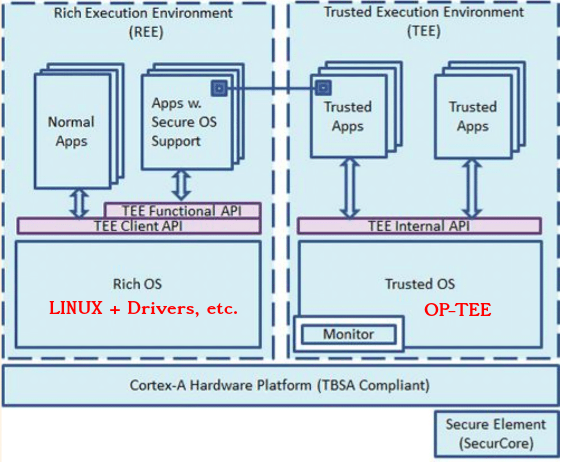
\includegraphics[width=0.6\columnwidth]{TZ-OP-TEE.png}
 \caption{ARM Cortex A: Normal world runs Linux, Trusted world runs OP-TEE.}\label{fig:tz}
\end{figure}


\subsection{Deliverables}
%Labs are in the format of capture-the-flag (CTF).
%You finish a task and retrieve a flag for that particular task.
%You will submit flags you captured in this lab to the corresponding questions on \verb|MyCourses|. 
%{\color{white}CSEC-659-FLAG-LAB1-READ-0x9876}
Submit a lab report on \verb|MyCourses|. The report should have screenshots and clear answer to all questions.

\section{Assignments}

\begin{enumerate}
 \item Follow the instructions available at \url{https://optee.readthedocs.io/en/latest/building/gits/build.html}. This includes the installation of \verb|repo|, if you don't already have it, and pre-requisite packages. The installation process will  setup the environment in Figure~\ref{fig:tz} (with Normal World running Linux and Trusted World running \verb|OP-TEE|). Note that these instructions support builds targeting several platforms. In our case, the target platform is \verb|QEMU| (v7), i.e., a simulator rather than a real device.  

 \item  Open a terminal and change current directory to the build directory created within your \verb|OP-TEE| folder, for example \verb|cd ~/<optee folder path>/build| (this path varies depending on the location you chose for the \verb|OP-TEE| folder in step 1).

In this directory, type \verb|make run|.
The first time you type \verb|make run| it will take a while. It may also tell you that your installation is missing some pre-requisite package. If this happens, go ahead, install that package, and try \verb|make run| again. Repeat this until \verb|make run| succeeds. 
(pre-requisites can be found here : \url{https://optee.readthedocs.io/en/latest/building/prerequisites.html#prerequisites})

OBS: You can compile faster by parallelizing the compilation process using the -j parameter. Template :
\verb|make -j<number_of_cores> run| . Example using 8 cores : \verb|make -j8 run|



Once \verb|make run| succeeds, you will end up in the QEMU console and it will also spawn two UART consoles. One console containing the UART for secure world and one console containing the UART for normal world.

{\bf \color{red}You are supposed to see three terminals at this step. Take a screenshot that shows all three terminals.}

\item You will see that it stops waiting for input on the QEMU console. To continue, type \verb|c| in the QEMU console.
After this step, the QEMU device will keep booting. You will notice that Linux boot is shown in one the terminals.
When it stops, it will prompt you to login. 
Type \verb|root| to login as the root; there is no password.

{\bf \color{red}Type \verb|uname -a| to show the information of this Linux distribution. Take a screenshot.}

\item \verb|xtest| is a test suite built to test TrustZone. Type \verb|xtest -l 0| in the normal world to start testing. 
{\bf \color{red}Answer the following question: what do you see in the normal world and secure world terminals?} 

\item {\bf Modifying TrustZone Apps:}

\verb|xtest| runs several sample tests. However, you can also run individual examples. \verb|make run| pre-loads the compiled binaries of the examples in the directory \verb|/usr/bin|. In the normal world Linux terminal, type \verb|cd /usr/bin|, then type \verb|ls| to see the list of binaries in that directory.
\verb|OP-TEE| example executable names start with \verb|optee_example_|. A description of the examples is available at \url{https://optee.readthedocs.io/en/latest/building/gits/optee_examples/optee_examples.html}.

Within the \verb|/etc/bin| directory, type \verb|./optee_example_hello_world|. This will run the example program.

{\bf \color{red}Answer the following question: what do you see in the normal world and secure world terminals?} 

Now you are going to modify the behavior of the hello world program by modifying its source code. At this point you can close all three (QEMU, normal world, secure world) terminals.

In your host machine, you will be able to find the source code of the Hello World example at:

\begin{itemize}
 \item Normal world: \verb|~/<optee folder path>/optee_examples/hello_world/host/main.c|
 \item Secure world: \verb|~/<optee folder path>/optee_examples/hello_world/ta/hello_world_ta.c|
\end{itemize}


\textbf{Your task is to modify both of these files such that:\\}

\begin{itemize}
 \item Normal world prints your full name;
 \item Instead of 42, normal world APP gives the \verb|ASCII| 
encoding of the first letter of your first name to the trusted world APP;
 \item Instead of incrementing the received number by 1, trusted world APP should increment it by 5.\\

\end{itemize} 

Once you are done with your changes to these files, you can go into \verb|~/<optee folder path>/build| directory and type \verb|make run| again.
It will build your changes and load the updated executable into \verb|/usr/bin| folder of the normal world Linux terminal.

{\bf \color{red} In the normal world terminal, type \verb|/usr/bin/optee_example_hello_world| to run your modified TrustZone app. Take a screenshot of both normal world and secure world terminals. The result should reflect your changes to the behavior of the hello world APP (Normal world prints your name, the number corresponds to the first letter of your name, and it gets incremented by 5 by the secure world counterpart).}


This exercise illustrates how to modify TrustZone apps in \verb|OP-TEE|. You can use these general steps to modify any TrustZone example APP at will, by changing its untrusted and trusted counterparts. Feel free to explore other cases and available example APPs. This will be useful should you decide to use TrustZone in your final research project.



\item {\bf Adding a new funtionality to hello world:}

One of the essential features of TrustZone is the ability to isolate and protect the memory of the secure world from the normal world. The most common usage for this is to store secrets and do cryptography operations inside the secure world without leaking any information to the normal world. Your task is to create two new functionalities for the hello world application: encryption and decryption. You will use the RSA algorithm to encrypt the message $msg$. The encryption function of RSA is the following :

\begin{equation}
	enc = msg^E\, mod \, N;
\end{equation}

And the decryption function:
\begin{equation}
	msg = enc^D \, mod \, N;
\end{equation}

Where the public key is $K_{pub}=(D=41, N=133)$, and the private key is $K_{priv}=(E=29, N=133)$. \textbf{In this work, the value of $msg$ is your RIT ID number}. To add the functionalities, you are expected to modify three files:

1. File \textbf{hello\_world\_ta.h} : Define two new IDs as shown bellow: 

\begin{lstlisting}
//<optee_path>/out-br/build/optee_examples_ext-1.0/hello_world/ta/include/hello_world_ta.h
...
/* The function IDs implemented in this TA */
#define TA_HELLO_WORLD_CMD_INC_VALUE		0
#define TA_HELLO_WORLD_CMD_DEC_VALUE		1
// ADD THE TWO LINES BELLOW 
#define TA_ENCRYPT 							2
#define TA_DECRYPT 							3
...
\end{lstlisting}

2. File \textbf{hello\_world\_ta.c} : implement two new functions \verb|tee_encrypt()| and \verb|tee_decrypt()|. The function  \verb|tee_encrypt()| must receive $msg$ inside the struct \textbf{TEE\_Param} and replace its value for its encrypted value $enc$. The function  \verb|tee_decrypt()| must receive $enc$ inside the struct \textbf{TEE\_Param} and replace its value for its decrypted value $msg$. \textbf{DELIVERY: For each function you will need to print its input and output values ($msg$ and $enc$). All the printed messages must appear in the secure world terminal.}. The header template of each function are:
(TIPS: You can follow the structure of the functions inc\_value() and dec\_value() to implement your functions. Try to understand what the hello world code do before hand and then "modify" these functions with the new functionalities)

\begin{lstlisting}
// <optee_path>/optee_examples/hello_world/ta/hello_world_ta.c
...
static TEE_Result tee_encrypt(uint32_t param_types,TEE_Param params[4]){
// CODE HERE
}
...
static TEE_Result tee_decrypt(uint32_t param_types,TEE_Param params[4]){
// CODE HERE
}
...
\end{lstlisting}

You also need to modify the entry point of the secure world to be able to call the functions above.

\begin{lstlisting}
// <optee_path>/optee_examples/hello_world/ta/hello_world_ta.c
...
TEE_Result TA_InvokeCommandEntryPoint(void __maybe_unused *sess_ctx,
			uint32_t cmd_id,
			uint32_t param_types, TEE_Param params[4])
{
	(void)&sess_ctx; 

	switch (cmd_id) {
	// ADD THE TWO CASES BELLOW
	case TA_ENCRYPT : 
		return tee_encrypt(param_types, params);
	case TA_DECRYPT : 
		return tee_decrypt(param_types, params);
	case TA_HELLO_WORLD_CMD_INC_VALUE:
		return inc_value(param_types, params);
	case TA_HELLO_WORLD_CMD_DEC_VALUE:
		return dec_value(param_types, params);
	default:
		return TEE_ERROR_BAD_PARAMETERS;
	}
}
...
\end{lstlisting}

3. File \textbf{main.c} : The main file of this example runs in the normal world. You will have to modify the main file to call the encryption and decryption functions that are inside the secure world to encrypt and then decrypt your RIT ID.  \textbf{DELIVERY: You will have to print the values of $msg$ before encryption, after decryption, and the value of the encrypted message $enc$. The prints must appear in the normal world terminal}.

\begin{lstlisting}
// <optee_path>/optee_examples/hello_world/host/main.c
\end{lstlisting}


\newpage
\textbf{You have to delivery ...}

\begin{itemize}
	\item All three modified files (add comments to your code please).
	\item Your RIT ID and the encrypted value of it.
	\item Screenshot of the secure world and normal world terminal with all the information that was asked (tagged with: \textbf{DELIVERY}).
\end{itemize}


\end{enumerate}






\end{document}
